% !TEX encoding = IsoLatin9

%%%%%%%%%%%%%%%%%%%%% SECTION 1
\section{Adresse et pointeurs}
\begin{frame}
  \begin{columns}
    \column{4.8cm}
    \tableofcontents[currentsection,hideothersubsections]
    \column{7cm}
      \centering{
      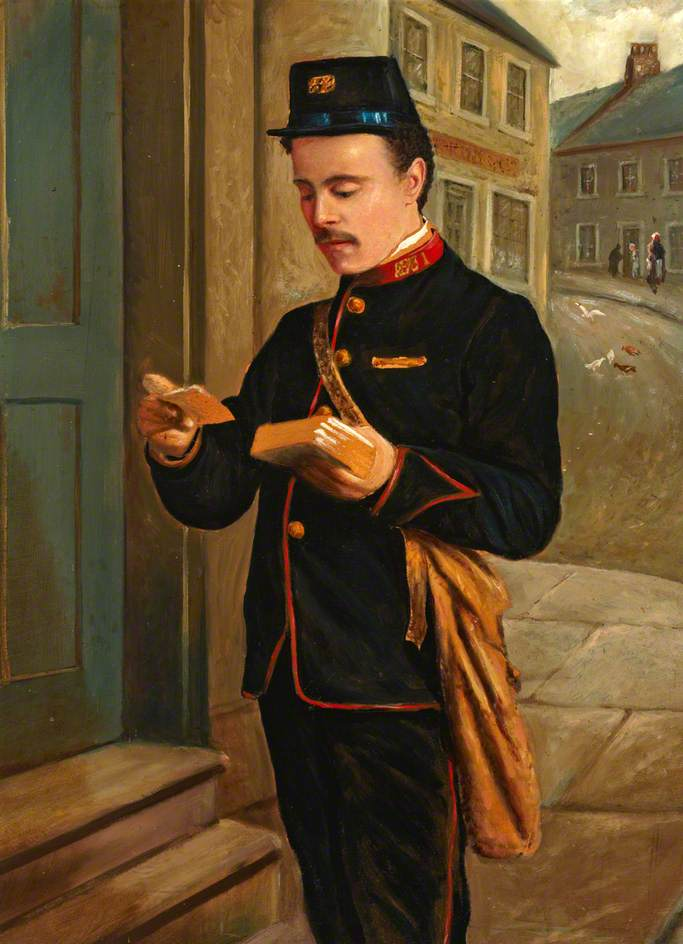
\includegraphics[width=5cm]{fig/postman.jpg}

      \hfill \textit{Portrait of a Postman} (vers 1900-1912 ??)\\
      \hfill Thomas Patterson \\
      \hfill The British Postal Museum \& Archive
    }
  \end{columns}
  
\end{frame}

\begin{frame}[fragile]
\frametitle{Variable et adresse m�moire}
\begin{block}{}
La m�moire d'un ordinateur est organis�e en suite de cases rep�r�es par 
une adresse.
\begin{itemize}
\item Chaque case m�moire a une adresse et un contenu.
\end{itemize}
\end{block}

Les variables d'un programme sont stock�es en m�moire et poss�dent
une valeur.


\begin{columns}
\column{0.2\textwidth}

\begin{codeblock}{}
\vspace{-.3cm}
\lstset{escapeinside={��}}
\lstset{basicstyle=\scriptsize}
\begin{codeC}
int n=3;
\end{codeC}
\vspace{-.3cm}
\end{codeblock}
\end{columns}
\vspace{1em}
\begin{columns}
\column{0.6\textwidth}

\begin{tabular}{|l|c|c|c|c|c|}
\hline
Adresse & ... & 4584 & 4585 & 4586 & ...\\
\hline
Valeur & ... &     & 3 & & \\
\hline
\multicolumn{3}{c}{} & \multicolumn{1}{c}{\Verb|n|}& \multicolumn{2}{c}{}\\
\end{tabular}

\column{0.35\textwidth}
\Verb|n| est � l'adresse 4585

\end{columns}
\end{frame}

\begin{frame}[fragile]
\frametitle{L'op�rateur \textcolor{bluegreen}{\&}}

\begin{block}{}
L'op�rateur \bvrb|&| permet de retrouver l'adresse d'une variable.
\end{block}

\begin{columns}
\column{0.2\textwidth}

\begin{codeblock}{}
\vspace{-.3cm}
\lstset{escapeinside={��}}
\lstset{basicstyle=\scriptsize}
\begin{codeC}
int n=3;
\end{codeC}
\vspace{-.3cm}
\end{codeblock}
\end{columns}

\vspace{1em}
\centering
\begin{tabular}{|l|c|c|c|c|c|}
\hline
Adresse & ... & 4584 & 4585 & 4586 & ...\\
\hline
Valeur & ... &     & 3 & & \\
\hline
\multicolumn{3}{c}{} & \multicolumn{1}{c}{\Verb|n|}& \multicolumn{2}{c}{}\\
\end{tabular}
\vspace{1em}

\begin{tabular}{ll}
\Verb|n| & contient 3 \\
\Verb|&n| & contient 4585 \\
\end{tabular}

\end{frame}

\begin{frame}[fragile]
\frametitle{Les pointeurs}
\begin{block}{}
Un pointeur est une variable contenant l'adresse d'une case m�moire.
\end{block}
\begin{itemize}
\item D�claration :\\
\vspace{0.5em}
\begin{columns}
\column{0.2\textwidth}
\begin{codeblock}{}
\vspace{-.3cm}
\lstset{escapeinside={��}}
\lstset{basicstyle=\scriptsize}
\begin{codeC}
int *pn;
\end{codeC}
\vspace{-.3cm}
\end{codeblock}

\column{0.75\textwidth}
\begin{tabular}{|l|c|c|c|c|c|c|}
\hline
Adresse & ... & 4584 & 4585 & 4586 & ...&6208\\
\hline
Valeur & ... &     & 3 & & &\\
\hline
\multicolumn{3}{c}{} & \multicolumn{1}{c}{\Verb|n|}& \multicolumn{2}{c}{} &\multicolumn{1}{c}{\Verb|pn|}\\
\end{tabular}

\end{columns}

\item Affection :\\
\vspace{0.5em}
\begin{columns}
\column{0.2\textwidth}
\begin{codeblock}{}
\vspace{-.3cm}
\lstset{escapeinside={��}}
\lstset{basicstyle=\scriptsize}
\begin{codeC}
pn = &n ;
\end{codeC}
\vspace{-.3cm}
\end{codeblock}

\column{0.75\textwidth}
\begin{tabular}{|l|c|c|c|c|c|c|}
\hline
Adresse & ... & 4584 & 4585 & 4586 & ...&6208\\
\hline
Valeur & ... &     & 3 & &  & 4585\\
\hline
\multicolumn{3}{c}{} & \multicolumn{1}{c}{\Verb|n|}& \multicolumn{2}{c}{} &\multicolumn{1}{c}{\Verb|pn|}\\
\end{tabular}

\end{columns}

\end{itemize}
\end{frame}

\begin{frame}[fragile]
\frametitle{L'op�rateur \bvrb|*|}
\begin{block}{}
\begin{itemize}
\item L'op�rateur \bvrb|&| permet de retrouver l'adresse d'une variable.\\
\item L'op�rateur \bvrb|*| permet de retrouver le contenu d'une adresse m�moire. (Op�ration de d�r�f�rencement)\\
\end{itemize}
\end{block}
\centering
\begin{tabular}{|l|c|c|c|c|c|c|}
\hline
Adresse & ... & 4584 & 4585 & 4586 & ...&6208\\
\hline
Valeur & ... &     & 3 & &  & 4585\\
\hline
\multicolumn{3}{c}{} & \multicolumn{1}{c}{\Verb|n|}& \multicolumn{2}{c}{} &\multicolumn{1}{c}{\Verb|pn|}\\
\end{tabular}
\vspace{1em}

\begin{columns}
\column{0.27\textwidth}
\begin{tabular}{ll}
\Verb|n| & contient 3 \\
\Verb|pn| & contient 4585
\end{tabular}

\column{0.27\textwidth}
\begin{tabular}{ll}
\Verb|&n| & contient 4585 \\
\Verb|*pn| & contient 3
\end{tabular}

\column{0.35\textwidth}
\begin{exampleblock}{}
Les �galit�s suivantes sont vraies :\\
\Verb|n == *pn|\\
\Verb|pn == &n | 
\end{exampleblock}

\end{columns}

\end{frame}

\begin{frame} [fragile]
 \setbeamercovered{transparent=30}
\frametitle<1>{Manipulation des pointeurs}
\frametitle<2>{Autre Notation}
\begin{columns}
\column{0.3\textwidth}
\begin{codeblock}{}
\vspace{-.3cm}
\lstset{escapeinside={��}}
\lstset{basicstyle=\scriptsize}
\begin{codeC}
int x=1, y=2, z=3 ;
\end{codeC}
\vspace{-.3cm}
\end{codeblock}

\column{0.63\textwidth}
\begin{tabular}{|l|c|c|c|}
\hline
\uncover<1> {Adresse & 2158 & 2159 & 2160} \\
\hline
Valeur &\visible<2>{1}&\visible<2>{2}&\visible<2>{3}\\
\hline
\multicolumn{1}{c}{} & \multicolumn{1}{c}{\Verb|x|}& \multicolumn{1}{c}{y} &\multicolumn{1}{c}{\Verb|z|}\\
\end{tabular}

\end{columns}
\hrulefill


\begin{columns}
\column{0.3\textwidth}
\begin{codeblock}{}
\vspace{-.3cm}
\lstset{escapeinside={��}}
\lstset{basicstyle=\scriptsize}
\begin{codeC}
int *p = &x ;
\end{codeC}
\vspace{-.3cm}
\end{codeblock}

\column{0.63\textwidth}
\begin{tabular}{|l|c|c|c|c|}
\hline
\uncover<1> {Adresse & 2158 & 2159 & 2160 & 2161} \\
\hline
Valeur &\visible<2>{1\tmark{v1}}&\visible<2>{2}&\visible<2>{3} & \visible<2>{\uncover<1>{2158\tmark{p1}}}\\

\hline
\multicolumn{1}{c}{} & \multicolumn{1}{c}{\Verb|x|}& \multicolumn{1}{c}{y} &\multicolumn{1}{c}{\Verb|z|} &\multicolumn{1}{c}{\Verb|p|} \\
\end{tabular}

\end{columns}
\hrulefill

\begin{columns}
\column{0.3\textwidth}
\begin{codeblock}{}
\vspace{-.3cm}
\lstset{escapeinside={��}}
\lstset{basicstyle=\scriptsize}
\begin{codeC}
y = *p ;
\end{codeC}
\vspace{-.3cm}
\end{codeblock}

\column{0.63\textwidth}
\begin{tabular}{|l|c|c|c|c|}
\hline
\uncover<1> {Adresse & 2158 & 2159 & 2160 & 2161} \\
\hline
Valeur &\visible<2>{1\tmark{v2}}&\visible<2>{1}&\visible<2>{3} & \visible<2>{\uncover<1>{2158\tmark{p2}}} \\

\hline
\multicolumn{1}{c}{} & \multicolumn{1}{c}{\Verb|x|}& \multicolumn{1}{c}{y} &\multicolumn{1}{c}{\Verb|z|} &\multicolumn{1}{c}{\Verb|p|} \\
\end{tabular}

\end{columns}
\hrulefill


\begin{columns}
\column{0.3\textwidth}
\begin{codeblock}{}
\vspace{-.3cm}
\lstset{escapeinside={��}}
\lstset{basicstyle=\scriptsize}
\begin{codeC}
*p = 0 ;
\end{codeC}
\vspace{-.3cm}
\end{codeblock}

\column{0.63\textwidth}
\begin{tabular}{|l|c|c|c|c|}
\hline
\uncover<1> {Adresse & 2158 & 2159 & 2160 & 2161} \\
\hline
Valeur &\visible<2>{0\tmark{v3}}&\visible<2>{1}&\visible<2>{3} & \visible<2>{\uncover<1>{2158\tmark{p3}}} \\

\hline
\multicolumn{1}{c}{} & \multicolumn{1}{c}{\Verb|x|}& \multicolumn{1}{c}{y} &\multicolumn{1}{c}{\Verb|z|} &\multicolumn{1}{c}{\Verb|p|} \\
\end{tabular}

\end{columns}
\hrulefill

\begin{columns}
\column{0.3\textwidth}
\begin{codeblock}{}
\vspace{-.3cm}
\lstset{escapeinside={��}}
\lstset{basicstyle=\scriptsize}
\begin{codeC}
p =&z ;
\end{codeC}
\vspace{-.3cm}
\end{codeblock}

\column{0.63\textwidth}
\begin{tabular}{|l|c|c|c|c|}
\hline
\uncover<1> {Adresse & 2158 & 2159 & 2160 & 2161} \\
\hline
Valeur &\visible<2>{0}&\visible<2>{1}&\visible<2>{3\tmark{v4}} &\visible<2>{\uncover<1>{2160\tmark{p4}}} \\

\hline
\multicolumn{1}{c}{} & \multicolumn{1}{c}{\Verb|x|}& \multicolumn{1}{c}{y} &\multicolumn{1}{c}{\Verb|z|} &\multicolumn{1}{c}{\Verb|p|} \\
\end{tabular}

\end{columns}


\begin{tikzpicture}[remember picture,overlay, auto,
 line/.style     = { draw, thick, color=black},
]
\begin{scope} [every path/.style=line]
\path <2-> ($(p1) + (-0.3,0)$) edge[bend right, *->] (v1) ;
\path <2-> ($(p2) + (-0.3,0)$) edge[bend right, *->] (v2) ;
\path <2-> ($(p3) + (-0.3,0)$) edge[bend right, *->] (v3) ;
\path <2-> ($(p4) + (-0.3,0)$) edge[bend right, *->] (v4) ;


\end{scope}
\end{tikzpicture}

\end{frame}

\begin{frame}[fragile]
\frametitle{Autre exemple}

\begin{columns}
\column{0.6\textwidth}
\begin{codeblock}{}
\vspace{-.3cm}
\lstset{escapeinside={��}}
\lstset{basicstyle=\scriptsize}
\begin{codeC}
#include <stdio.h>

int main() 
{
   int u1, u2, v=3;
   int *p1;
   int *p2;
   u1 = 2*(v+5);
   p1 = &v;
   p2 = p1;
   *p2 = 5;
   p2=&u1;
   u2 = 2*(*p1+5);
   *p2=*p2+1:
   printf("\nu1=%d u2=%d v=%d",u1,u2,v);
   return (0);
}
\end{codeC}
\vspace{-.3cm}
\end{codeblock}
\column{0.29\textwidth}
\begin{termblock}{Test d'ex�cution}
%\vspace{-.3cm}
\lstset{escapeinside={��}}
\lstset{basicstyle=\scriptsize}
\begin{lstlisting}
u1=... u2=... u3=...
\end{lstlisting}
\vspace{-.3cm}
\end{termblock}


\end{columns}
\end{frame}